% Copyright 2021 Thomas Ascher
% SPDX-License-Identifier: CC-BY-SA-4.0

\documentclass[a4paper,parskip=half]{scrartcl}

\usepackage[T1]{fontenc}
\usepackage[ngerman]{babel}
\usepackage{csquotes}
\usepackage[regular,condensed,sfdefault]{roboto}
\usepackage{booktabs}
\usepackage{graphicx}
\usepackage{float}
\usepackage[hidelinks,pdfencoding=auto,
  pdfauthor={Thomas Ascher},
  pdfusetitle,
  pdfkeywords={Grainfather,Conical Fermenter,Pro Controller}]{hyperref}
\usepackage{microtype}

\addto\extrasngerman{
\def\figureautorefname{Abb.}
\def\tableautorefname{Tab.}
\def\equationautorefname{Gl.}
}

\addto\captionsngerman{
\renewcommand{\figurename}{Abb.}
\renewcommand{\tablename}{Tab.}
}

\title{Grainfather Conical Fermenter Pro Controller}
\author{Thomas Ascher <thomas.ascher@gmx.at>}
\date{11. Oktober 2021, \href{http://creativecommons.org/licenses/by-sa/4.0/}{CC BY-SA 4.0}}

\begin{document}
\maketitle

\section*{Einleitung}

Zusammen mit der neuesten Generation des Conical Fermenters
hat Grainfather für die vorherige Geräterevision ein Upgrade
in der Form des Grainfather Conical Fermenter Pro Controllers (\autoref{fig:package}) für rund € 99 auf den Markt gebracht.
Die wesentlichen Verbesserungen dieses Upgrades werden im Rahmen
dieses Artikels vorgestellt. 
 
\begin{figure}[h]
\centering
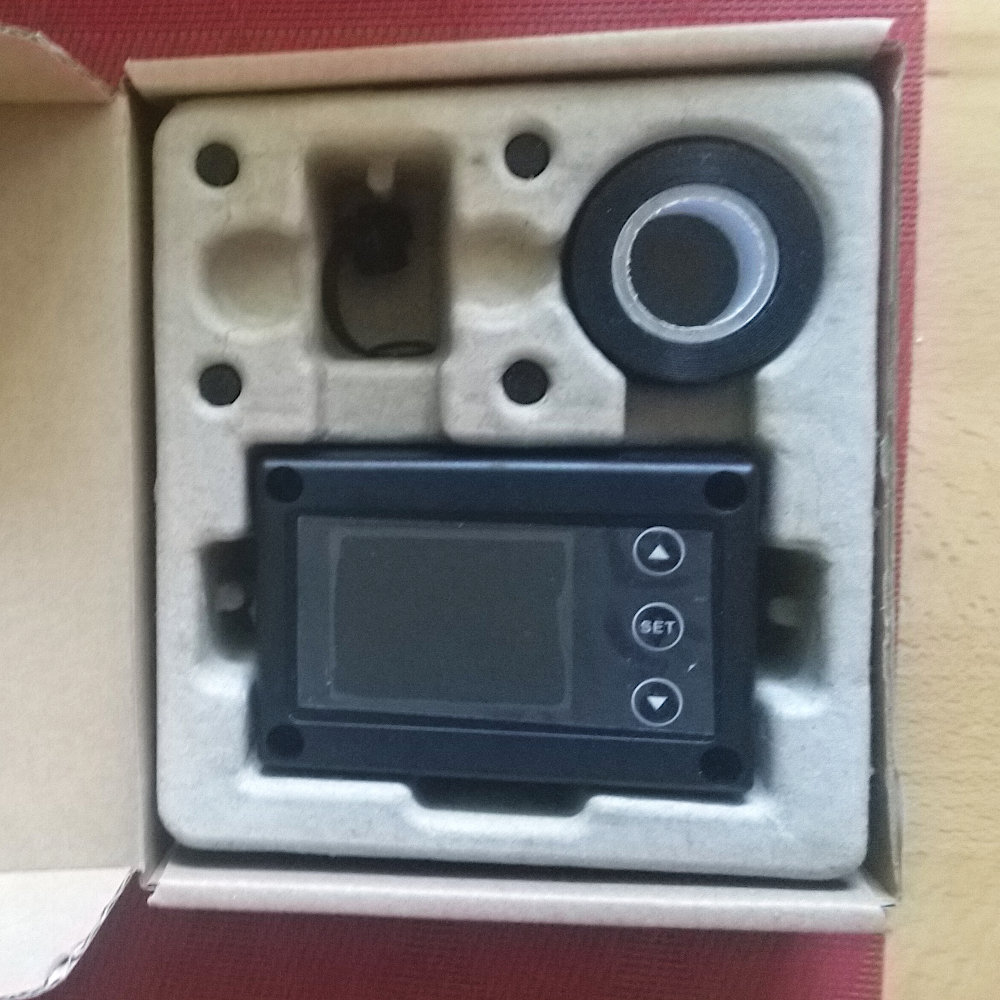
\includegraphics[width=4.8cm]{images/gfpc_package.jpg}
\caption{Lieferumfang des Pro Controllers (Ascher, 2021)}
\label{fig:package}
\end{figure}

\section*{Verbesserungen im Überblick}

Neben der Internetanbindung an die Grainfather Community
via WLAN zur Fernsteuerung und Messdatenaufzeichung kann der
Pro Controller auch mit einigen Detailverbesserungen aufwarten.
Das sind unter anderem ein Farbdisplay und eine Anpassung
der einzelnen Menüdarstellung (\autoref{fig:displaynewmain},
\autoref{fig:displayoldmain}). Darüber hinaus ist der neue
Controller wasserdicht und kann nach der Montage nicht
wie sein Vorgänger einfach abgenommen werden.
Während sich beim alten Controller noch vier fixe Gärprofile mit
maximal fünf Temperaturstufen konfigurieren lassen, können nun
auch neue Profile mit maximal sechs Stufen angelegt werden.

\begin{figure}[H]
\centering
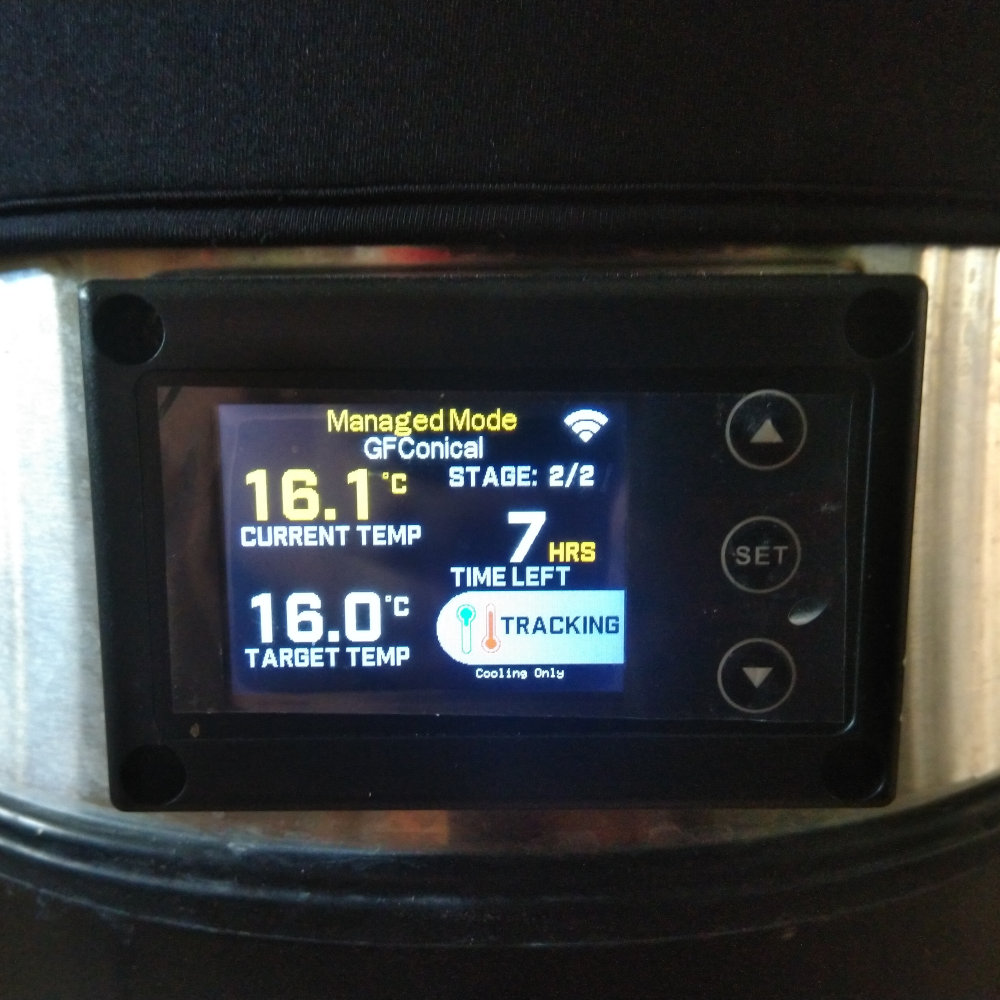
\includegraphics[width=4.8cm]{images/gfpc_display_new_main.jpg}
\caption{Pro Controller Display (Ascher, 2021)}
\label{fig:displaynewmain}
\end{figure}

\begin{figure}[H]
\centering
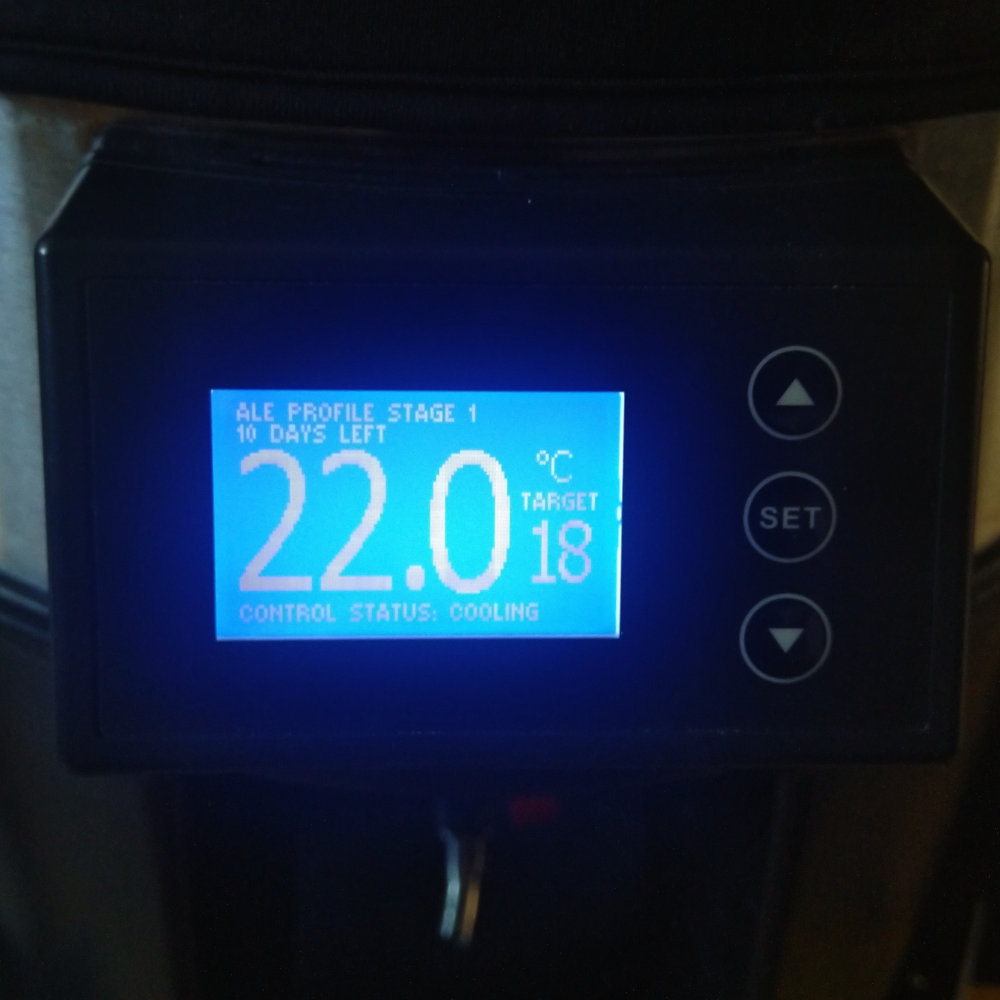
\includegraphics[width=4.8cm]{images/gfpc_display_old_main.jpg}
\caption{Altes Controller Display (Ascher, 2021)}
\label{fig:displayoldmain}
\end{figure}

Die Software des Pro Controllers lässt sich per Firmware Update
aktualisieren. Seit der Veröffentlichung wurden bereits zwei
neue Funktionen nachgeliefert, das sind die Möglichkeit den
gemessenen Temperaturwert zu kalibrieren und eine Warnung
bei Unterschreitung der Regeltemperatur auszugeben.

\section*{Anbindung an die Grainfather Community}

Zur Nutzung der Online-Funktionen des Pro Controllers wird ein
kostenfreies Grainfather Community Konto und die Grainfather
Community App (GF Connect) für Android oder iOS vorausgesetzt.
Das initiale Pairing zwischen WLAN und Konto erfolgt über die App.
Danach kann der Zugriff entweder über die App oder durch die
Webseite \url{https://community.grainfather.com} erfolgen.

Die Grainfather Community enthält einen vollständigen
Braurechner. Die Anbindung des Conical Fermenters ist
im Rahmen dessen Workflows integriert (\autoref{fig:integration}).
Dafür muss erst ein Rezept im Braurechner erstellt oder
via BeerXML importiert und ein neuer Brauvorgang gestartet werden.
Spezielle Importe sind für BeerSmith, Brewer's Friend und
Brewfather realisiert. Während der Gärphase kann
durch die Betätigung den Schalters „Manager Mode“ das
Gärprofil des Rezepts an den Pro Controller übertragen werden.

Neben der Übertragung der Gärprofile lassen sich auch
Messdaten (Temperatur und scheinbarer Restextrakt) innerhalb von Grainfather Community aufzeichnen und ebenfalls als CSV Datei herunterladen. Dabei werden neben dem Pro Controller folgende
Geräte unterstützt:
\begin{itemize}
\item \href{https://brewbrain.nl}{Brewbrain Float Hydrometer}
\item \href{https://www.ispindel.de}{iSpindel}
\item \href{https://plaato.io/products/plaato-airlock}{PLAATO Airlock} 
\item \href{https://tilthydrometer.com}{Tilt Hydrometer}
\end{itemize}

Für die Einrichtung der zusätzlichen Messgeräte beinhaltet
der Braurechner entsprechende Hilfetexte. Für das
Tilt Hydrometer wird während der gesamten Aufzeichnungszeit ein
zusätzliches Android oder iOS Gerät oder Tilt Pi benötigt.
Beim Float Hydrometer  ist im Brewbrain Konto die Grainfather
Integration zu aktivieren.

Auf Basis der aufgezeichneten Messdaten und der verstrichenen
Gärzeit ist es möglich Benachrichtigungen zu konfigurieren
(\autoref{fig:notification}). Ein Beispiel hierfür ist
die Zusendung einer E-Mail nach Erreichung
eines definierten scheinbaren Restextrakts.

\begin{figure}[H]
\centering
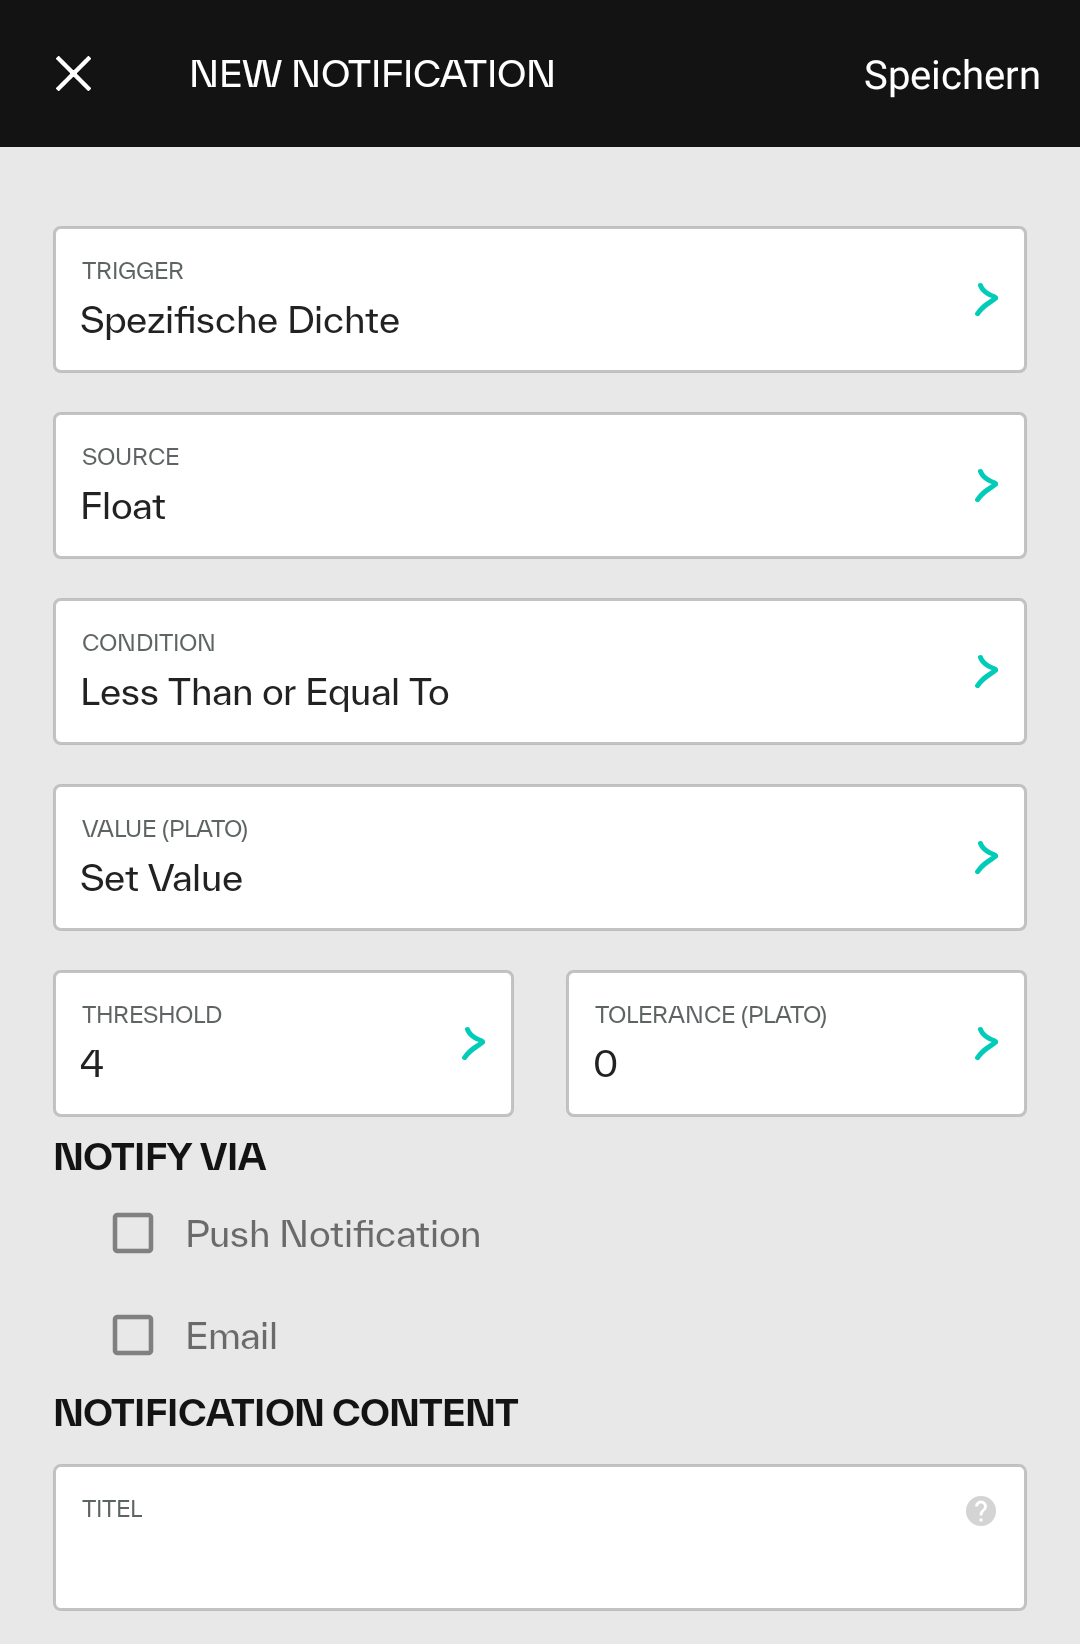
\includegraphics[width=4.8cm]{images/gfpc_notification.png}
\caption{Konfiguration von Benachrichtigungen (Ascher, 2021)}
\label{fig:notification}
\end{figure}

\begin{figure}[H]
\centering
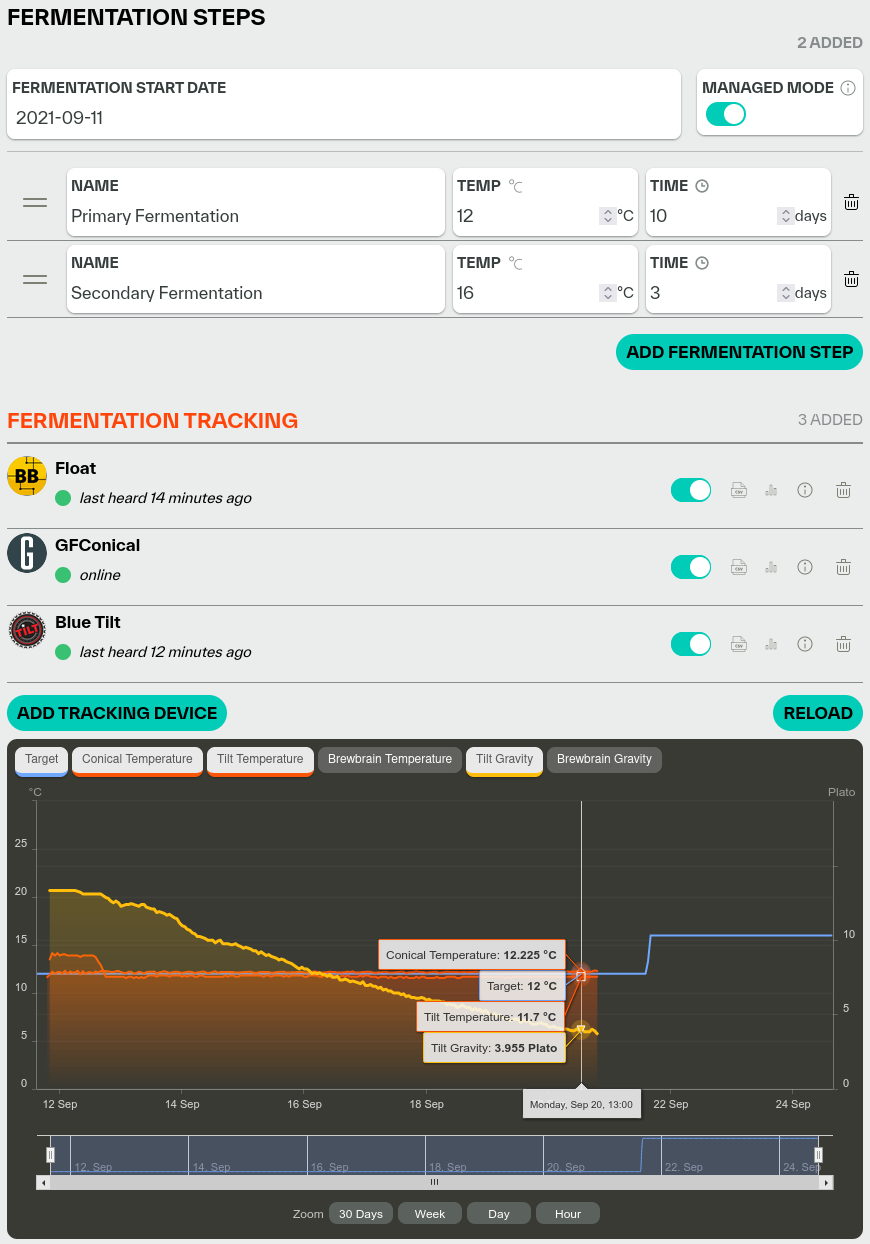
\includegraphics[width=14.4cm]{images/gfpc_integration.png}
\caption{Integration in Grainfather Community (Ascher, 2021)}
\label{fig:integration}
\end{figure}

\section*{Umbau}

Der Umbau auf den Pro Controller gestaltet sich einfach. Es
wird dafür lediglich ein Kreuzschraubenzieher benötigt.
Nach dem Abnehmen des alten Controllers kann die Deckplatte
abgeschraubt und die daran befestigten Steckverbinder
gelöst werden (\autoref{fig:installold}). Die Stecker des
Pro Controllers sind dann wie in \autoref{fig:installnew}
gezeigt wieder zu verbinden. Dabei ist auf die farbliche
kodierung der einzelnen Leitungen zu achten.

\begin{figure}[H]
\centering
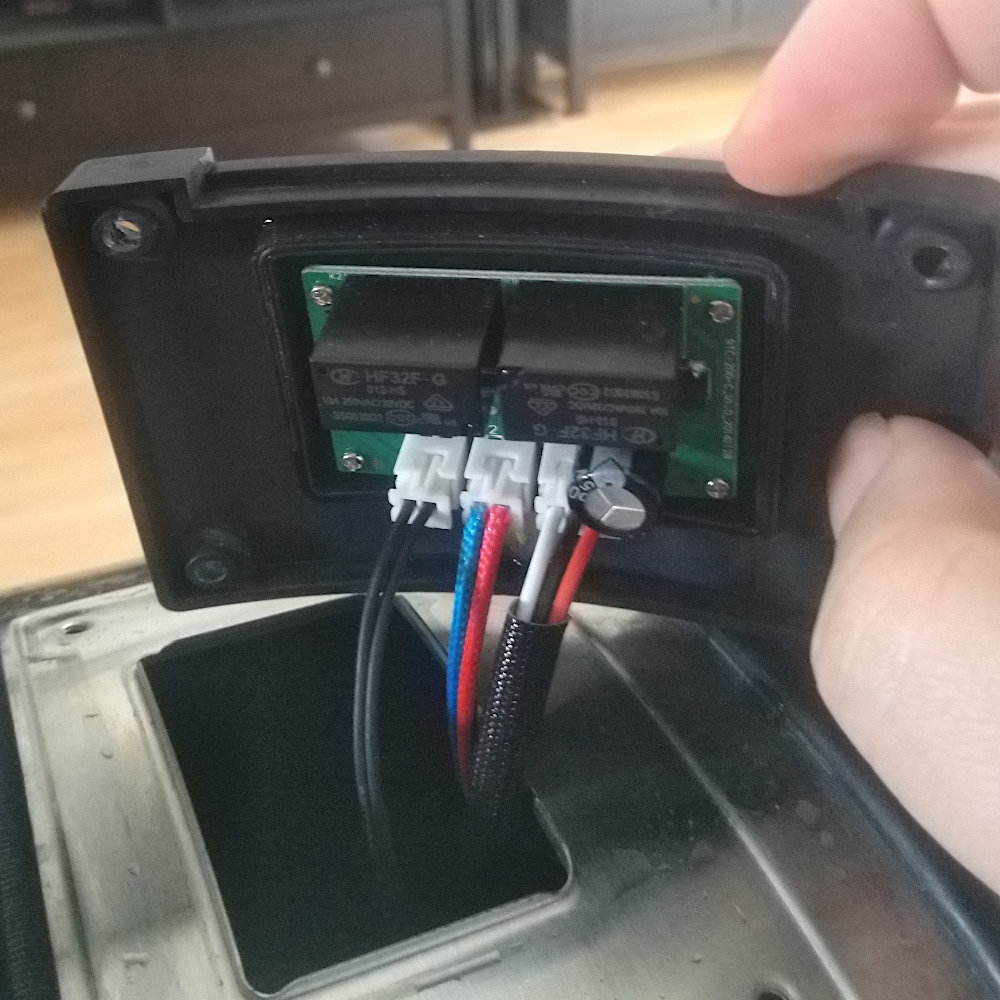
\includegraphics[width=4.8cm]{images/gfpc_install_old.jpg}
\caption{Ausbau alter Controller (Ascher, 2021)}
\label{fig:installold}
\end{figure}

\begin{figure}[H]
\centering
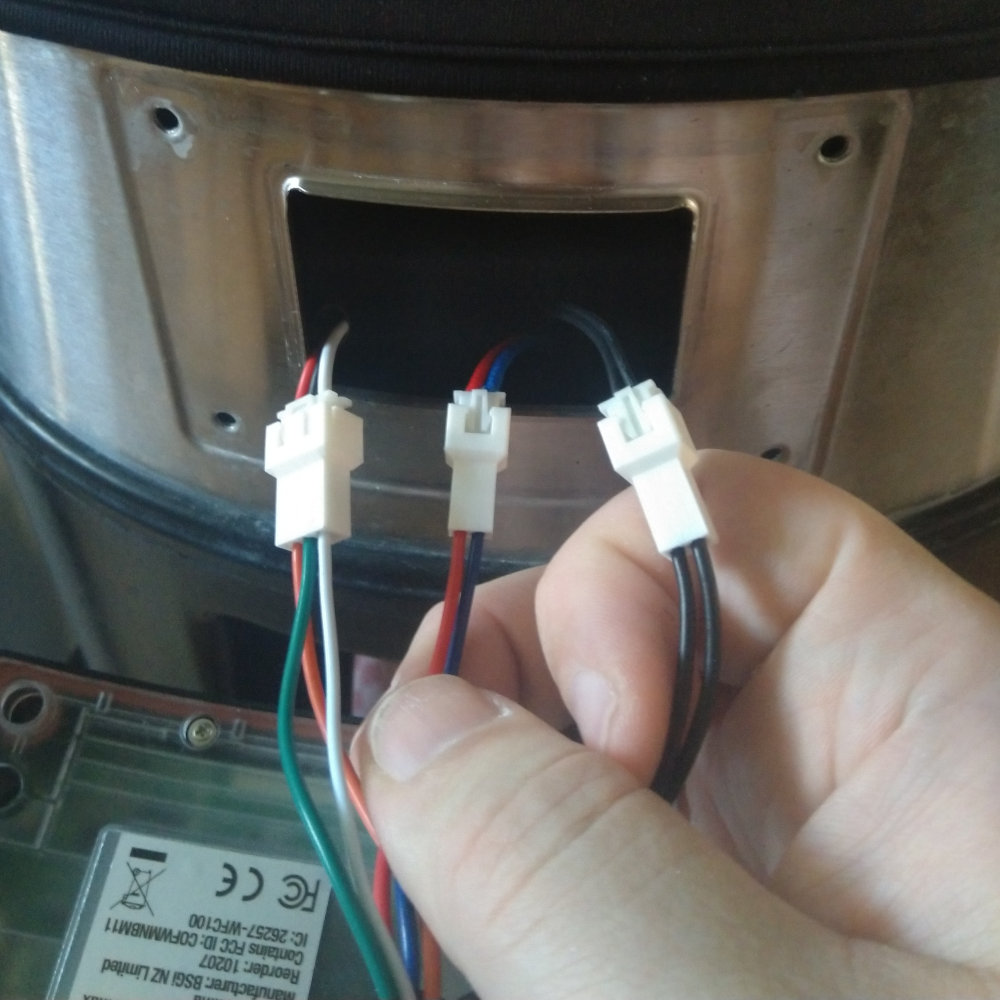
\includegraphics[width=4.8cm]{images/gfpc_install_new.jpg}
\caption{Einbau Pro Controller (Ascher, 2021)}
\label{fig:installnew}
\end{figure}

Im Lieferumfang des Pro Controllers (\autoref{fig:package})
befindet sich neben dem Controller selbst auch ein Isolierband
zur Isolierung der Steckverbindungen zum Schutz vor
Korrosion. Die beigelegten Stopfen verschließen die
Schraublöcher und den Stromanschluss des Conical Fermenters.

\section*{Resümee}



\end{document}